

\part{Weitere Werke}

\fancyhead[L]{\nouppercase{\lastrightmark}}



\begin{chapterbox}
    \chapter{Weitere wilde Werke eines Butterbrotbären}
    \label{Weitere wilde Werke eines Butterbrotbären}
    Andorische Fan-Werke meiner Wenigkeit, welche im Netz zu finden sind. Für eine vollständige Liste, siehe \url{https://legenden-von-andor.de/forum/viewtopic.php?p=116297\#p116297}.
\end{chapterbox}




{\parindent0pt



\az{diverse Jahre}

\section{Viel zu viele Fan-Held*innen (ab 2019)}

\begin{center}
    Fan-Held*innen aus der Taverne
\end{center}

\bildmitts[width=0.67\textwidth]{Heldencompilation.jpg}





\newpage


\section{Würfelerwartungswertberechnungen (ab 2019)}


\begin{center}
    Berechnungen aus der Taverne

    \url{https://legenden-von-andor.de/forum/viewtopic.php?p=110899#p110899}
\end{center}

\bildmitts[width=\textwidth]{Würfelerwartungswerte Icons.jpg}

\bildmitts[width=\textwidth]{Würfelerwartungswerte Zahlen.jpg}








\newpage
\section{Der Tolle Troll (2021)}

\begin{center}
    Fan-Held aus der Taverne

    \url{https://legenden-von-andor.de/forum/viewtopic.php?f=13&t=6119}
\end{center}

\bildmitts{Der Tolle Troll (2021).jpg}



\textbf{Ideen, Texte und Gestalltung:} Boggart, Butterbrotbär, Lost in the Echo und Schlafende Katze mit allerlei Impulsen vom Troll persönlich!\bigskip

Die Tavernengemeinschaft gratuliert dem ebenso rundum einzigartigen wie ideenreichen, Geschichten erzählenden, recht außergewöhnlichen Troll ganz herzlich zu 3000 Beiträgen hier im Forum!!!

Angesichts dieses außerordentlichen Anlasses konnten wir Anhänger der ausgezeichneten andorischen Allgemeinheit nicht davon absehen, als Anerkennung aller Aktivität und Arbeit dieses Auskenners einen frischen Fan-Helden anzufertigen.

Die Idee zur Willenspunkte-Vulnerabilität dieses Wesens haben wir womöglich von jemandem entwendet ;)

Im strahlend sonnigen Sommer, so sagt man, sieht man dieses sprachbegabte, selbstsichere Subjekt auf dem schönen Feld Sechs, sowohl beim souverän sarkastischen, schadenfrohen Scherzen als auch stundenlangem, sehr seriösen Schwafeln mit skeptischen, schreckhaft schüchternen, nach sicheren, schmalen Straßen suchenden Spaziergängern, beim schlauen Sinnieren über schlagfertige, stilbewusste Strategien sowie beim sinnlichen, schläfrigen Schnarchen im schattigen Schutz sanfter Sträucher.
Zur zwielichtigen, zeitweise zappendusteren (Winter-)Zeit zieht es diesen zuversichtlichen Zweibeiner zielstrebig zügig zum ziemlich zentralen Zugang einer Zwergenhöhle zurückliegender Zeiten, seinem zeitweilig zukünftigen Zuhause Feld Zwohundertneunzehn. Dort argumentiert er allabendlich mit allerlei anwesenden Argen in ausschweifenden Alliterationen über allgemeine Ausnahmen absurden Ausmaßes.

Karrenweise kommen kreuzende Kreaturen kurzum zu diesem Kenner kreativer Kurzgeschichten.
Viele Feinde finden völlig fälschlich Freude an Forns vielversprechend frohlockendem Freund.
Und wie bei Freund Forns Fähigkeit haben fesche Päsche fiese Folgen für freche Feinde.

\textbf{Dreitausend Dank an den tollen Troll im Namen aller Tavernengäste!!!}
\textbf{Die coole Creativ-Gaming-Force gegen chaotischen Covid-Frust.}

PS: Zu den lästigen Legenden der letzten Hoffnung liegen lauwarme Ideen vor.






\newpage
\section{Die Prinzessin von Andor (2021)}


\begin{center}
    Fan-Mini-Erweiterung aus der Taverne

    \url{https://legenden-von-andor.de/forum/viewtopic.php?f=8&t=6186}
\end{center}

\bildmitts{Die Prinzessin von Andor (2021).jpg}

\textbf{Erfinder*innen:} Boggart/Kar éVarin, Butterbrotbär,
Lost in the Echo, Schlafende Katze und Troll\bigskip

\textit{Es kam daher, vor langer Zeit,} \textit{ein Gast in die Taverne, ganz gescheit.}

\textit{Unbekannt waren Weg und Ziel,} \textit{wir wussten nur sein' Namen: Galaphil.}

\textit{In der Taverne, wohl bekannt,} \textit{leiht er stets eine helfende Hand.}

\textit{Und vor bald schon zwei Jahr',} \textit{brachte er die Idee des Stammtisches dar.}

\textit{Seitdem sind noch mehr bei Gilda zu Gast} \textit{und machen da mit Freuden Rast.}

\textit{Wir hoffen, es bleibt noch lange so,} \textit{und sind darüber äußerst froh.}

\textit{3000 Beiträge konntest du nun schon schreiben,} \textit{wir sind sicher, dabei wird es nicht bleiben.}

\textit{Und laut erschallt's in Andor noch,} \textit{der Galaphil, der lebe hoch!}








\newpage
\section{Kreaturenkarten statt Kreaturenplättchen (2023)}

\begin{center}
    Fan-Spielvariante aus der Taverne

    \url{https://legenden-von-andor.de/forum/viewtopic.php?f=8&t=9668}
\end{center}

\bildmitts{Kreaturenkarten (2023).jpg}
 

Wann immer ihr ein gewöhnliches Kreaturenplättchen ausführen würdet, zieht stattdessen zwei zufällige Kreaturenkarten und legt sie zufällig nebeneinander. Die beiden schwarzen Ziffern bestimmen das Zielfeld (falls dieses nicht existiert, wechselt die 10er-Stelle zur weißen Ziffer) und das einzige vollständige Symbol zwischen den beiden Karten gibt an, was auf dort erscheint (von links nach rechts). Danach werden die zwei Kreaturenkarten zurück in den Stapel gemischt.

Falls eine Kreatur durch Kreaturenkarten erscheinen sollte, aber es keine dieser Art mehr im Vorrat hat, erscheint stattdessen eine Kreatur der nächstschwächeren noch vorhandenen Art.

Falls eine Kreatur durch Kreaturenkarten auf ein Feld gestellt werden sollte, von dem kein Pfeil wegzeigt und/oder welches ein Kreaturen-Zielfeld ist (z.B. Rietburg, Lager der Tulgori oder Lager der Trolle), wird die Position dieser Kreatur stattdessen mit einem roten (10er-Stelle) und einem Heldenwürfel (1er-Stelle) ausgewürfelt, gegebenenfalls mehrfach.

Falls eine Kreatur durch Kreaturenkarten auf ein Feld gestellt wird, auf dem Bauern liegen, und von dem ein Pfeil wegzeigt, dürft ihr die Bauern auf das nächste kreaturenfreie Feld entlang der Pfeile versetzen.









\newpage
\section{ANDOR JUNIOR Erweiterungspaket (2020)}

\begin{center}
    Fan-Spielvariante aus der Taverne

    \url{https://legenden-von-andor.de/forum/viewtopic.php?f=8&t=5567}
\end{center}

\bildmitts{ANDOR JUNIOR Erweiterungspaket (2020).jpg}

\textbf{Erfinder*innen:} Schlafende Katze, Troll und Butterbrotbär

Kürzlich ist mir ein mysteriöses Paket per Falke zugestellt worden. Daran war ein Brief befestigt, welcher sich wie folgt anhört:

\textit{Dieses Andor-Junior-Fan-Erweiterungs-Paket besteht aus 11 Bonus-Helden, 9 Bonus-Aufgaben sowie einem Bonus-Endgegner.}

\textit{Die 11 Bonus-Helden sind Junior-Varianten der 11 noch nicht als Junior-Helden erschienenen offiziellen Helden (ausser Stinner). Jeder dieser Bonus-Helden ersetzt den offiziellen Junior-Helden seiner Würfelfarbe (bei Darh einer der drei). Prinzipiell könnt ihr aber auch mehrere Helden derselben Würfelfarbe gleichzeitig spielen, solange ihr im Voraus bestimmt, welcher Held welcher Heldenfarbe entspricht, wenn das für eine Aufgabe relevant sein sollte.}

\textit{Die 9 Bonus-Aufgaben können beliebig miteinander und mit den ursprünglichen Aufgaben gemischt werden. Sie benötigen oftmals Plättchen und Figuren aus dem Grundspiel oder einer Grundspiel-Erweiterung, diese können aber leicht ersetzt werden, falls ihr sie nicht besitzt.}

\textit{Mit dem neuen Endgegner könnt ihr euch nun endlich dem Drachen Tarok im Kampf stellen und die riesige Echse furchtlos vertreiben.}

\textit{Zu guter Letzt sei noch erwähnt, dass wir aus Gründen des Helden-Balancing empfehlen, bei der originalen Junior-Magierin gewürfelte Blitze als Fackeln zählen zu lassen.}

Spannend! Nur leider sieht es so aus, als hätte ein gewisser Schmierfink die Karten bereits vor mir in die Finger gekriegt und seine Meinung mit dunkler Tinte kundgetan.


\begin{center}
    Beiträge aus der Taverne

    "1. Tavernenstammtischparty!" (2020)
\end{center}

[Schlafende Katze:] Naja, eigentlich war ich ja schon die ganze Zeit da ;) Ich darf euch heute noch was zu Andor Ju...*\textbf{FAUCH!!!}*

[Varkur himself:] Muhahaha! :twisted: Seid gegrüßt, erbärmliches Gesindel! Habt ihr gedacht, ihr wäret mich los? Von Stund an werde ich sogar eure Kinder nicht mehr in Ruhe lassen! {\footnotesize Muhahahahaa! :twisted:}

[Towa:] Oh! Mit dem habe ich nicht gerechnet. Was willst du hier?

[Varkur himself:] Ich werde das Rietland brennen lassen! {\footnotesize Muhahahahaa! :twisted:}

[Tavernengaukler:] Der schon wieder... :x :o :lol:

[Varkur himself:] Schweig, Unwürdiger! Außer du willst um Gnade betteln. {\footnotesize Muhahahahaa! :twisted:}

[Lost In The Echo:] Varkur? Was hast du uns mitzuteilen? Sprich, bevor du aus diesem Ort des Friedens verstoßen wirst!

[Varkur himself:] Egal wer von euch sich mir in den Weg stellt, ob billiger Bettvorleger, wolfsvernarrter Wilder, würdelose Wasserplanscherin oder mickriger Möchtegernmensch: Ihr werdet scheitern! Ich kann es mit allen Helden aufnehmen! \textbf{ALLEN!} {\footnotesize Muhahahahaa! :twisted:}

Ich bin Varkur! Der mächtigste Dunkle Magier aller Zeiten! {\footnotesize Muhahahahaa! :twisted:}

Euch erwarten zahllose (neun) neue Herausforderungen: Torkelnde Trolle, aggressive Arbaks, fiese Fluggors... und meine Wenigkeit! Und selbst wenn ihr all das übersteht, wird es nicht mehr reichen, irgendwelche winselnden Welpen zu ihrer Mama zurückzuschleifen! Ihr werdet es mit Tarok persönlich aufnehmen müssen! :twisted: {\footnotesize Muhahahahaa! :twisted:}

[Lost In The Echo:] Da du ja scheinbar nicht an einer konstruktiven Unterhaltung interessiert bist, möchte ich in die Gruppe fragen, wer wohl mit dem billigen Bettvorleger gemeint ist : :?

[Varkur himself:] Der provisorische Pelzkragen natürlich... {\footnotesize Muhahahahaa! :twisted:}

[Schlafende Katze:] Was zu trinken? Oder doch lieber die Tür?

[Varkur himself:] Ein Rachenputzer … mit Olive. :) {\footnotesize Muhahahahaa! :twisted:}

[Schlafende Katze:] NARAVEN!!! Hast du noch was übrig von deinem Cocktail für unseren Gast?

[Boggart:] Einmal Thoraldmilch mit Olive, bitteschön! Wohl bekomms!

[Varkur himself:] Danke sehr. :P {\footnotesize Muhahahahaa! :twisted:}

[Varkur himself:] Ich habe schon genug Zeit in dieser verranzten Taverne verschwendet! Ich gehe wann ich will, nicht weil mich jemand vertreibt, das muss ich klarstellen. Aber ich werde wiederkommen! Ihr werdet gar nicht erst gegen den Drachen kämpfen, weil ihr davor an mir vorbeimüsst. An MIR!
Bis dann… {\footnotesize Muhahahahaa! :twisted:}

Muhahahaha! :twisted: *puff*

[Schlafende Katze:] Was ich eigentlich sagen wollte, bevor Varkur mich unterbrochen hat:

Der Troll, Butterbrotbär und ich haben uns ein bisschen mit Andor Junior beschäftigt.

Es sind \textbf{ALLE} offiziellen Helden jetzt spielbar und es gibt insgesamt neun neue Aufgaben.
Zusätzlich zu denen, die Varkur schon angedeutet hat gilt es Runensteine den Gors abzuluchsen, die Tulgori durch das Rietland zu begleiten und dem Trunkenen Troll unter die Arme zu greifen. Natürlich alles Kindgerecht!

Und als wäre das nicht genug, gibt es statt der Wolfssuche einen spannenden Drachenkampf am Schluss :)




\newpage
\az{Jahr 61}
\section{Arbon auf der Flucht (2021)}

\begin{center}
    Fan-Legende aus der Taverne

    \url{https://legenden-von-andor.de/forum/viewtopic.php?f=5&t=6396}
\end{center}

\bildmitts{Arbon auf der Flucht (2021).jpg}

\textbf{Erfinder*innen:} Butterbrotbär, Schlafende Katze, Troll

\textbf{Gestaltung:} Schlafende Katze

\textbf{Inhaltsangaben:} Diese Legende spielt nach dem Storytext „Die Geschichte des drittbesten Bogenschützen“ und vor dem Storytext „Die Hüterin und die Hexe“. Nachdem Arbon von Melkart, Pago und Folla in den Schwarzen Archiven überrascht wurde, befindet er sich nun auf der Flucht vor dem jungen Fährtenleser Fenn und den wütenden Bewahrern. In dieser Legende spielt einer der Mitspieler den Helden Arbon, der sich unsichtbar über das Spielfeld bewegt, während die Jäger sich auf die Suche nach ihm begeben. Dabei müssen sie den Verräter nicht nur finden, sondern auch zum Baum der Lieder zurück schleifen. Wenn nur die zusätzlichen Aufgaben und die vielen nervigen Gors nicht wären. Doch auch für Arbon ist die Flucht nicht leicht, denn scharfe Vogelaugen und die Jäger machen ihm das Leben schwer.

\textbf{Spielerzahl:} 2-4 Spieler

\textbf{Spielmaterial:} Grundspiel + Neue Helden

Erlebt ein unvergessliches (Schlafende-)Katz-und-Maus-Spiel quer durch Andor. Schwitzt mit Arbon, verzweifelt mit den Jägern und lasst euch nicht von unnötigen Storykarten irritieren!

\begin{center}
    Beiträge aus der Taverne

    "2. Tavernenstammtischparty 2021"
\end{center}

[Hogo:] für mich ein wasser, bitte. 
danke. mein gesicht ist sehr langweilig.

[Schlafende Katze:] Hogo, ein bisschen destruktiv eingestellt? Sooo hässlich bist du auch nicht :P

[Hogo:] hässlich ist auch nicht langweilig.

[Schlafende Katze:] mit Kapuze schwer zu beurteilen :P

[Hogo:] ja.

[Butterbrotbär:] Sind alle hier? Können wir loslegen? :D

[Hogo:] alle da! jetzt tür verriegeln und niemanden mehr reinlassen.

[...]

[AB von dem Andorwiki:] Hogo, beherrschst du die Handwerkkunst?

[Hogo:] nein. ich beherrsche gar nichts. beachtet mich nicht.

[Pago:] *In die Taverne stürz* Habt ihr ihn gesehen?
So einen jungen Barbar... Bisschen kleiner wie ich. Rote Haare. Rabe? Wenn, Denn, Venn... oder irgendwie so müsste er heißen. Ich hab eine Nachricht von ihm bekommen, dass er hier irgendwo wäre

[AB von dem Andorwiki:] Fenn?

[Pago:] Ja, genau so war der Name!!! Habt ihr ihn gesehen?

[Troll:] Nö, war schon seit 2016 (?) nicht mehr hier.

[Pago:] :shock: Das kann gar nicht sein! Ich habe ihn erst vor kurzem am Baum der Lieder getroffen, als er einen Auftrag angenommen hat.

[Butterbrotbär:] Wie kommst du denn darauf, dass Fenn hier wäre? Wollte er auch das Stammtisch-Jubiläum feiern?

[Pago:] Schön für euren Stammtisch. Dabei gibt es hier viel wichtigeres!!!

[Lost In The Echo:] Kannst du uns beschreiben, was er für Kleidung trug, als du ihn das letzte Mal gesehen hast?

[Pago:] Nunja. Keine Ahnung. Braun eben. Ist auch nicht so wichtig.... Wir hatten einige Schwierigkeiten am Baum der Lieder und Fenn sollte und bei der Suche nach einem verdächtigen Subjekt helfen
Ein mieser Verräter. Ehemals ein Wächter des Schwarzen Archivs. Hat Melkart mit einem Messer bedroht und ist dann abghauen. Arbon ist der Name dieses unwürdigen Stück Drecks...
Habt ihr wenigstens Kunde von IHM? Oder versteckt ihr ihn sogar in eurer Mitte?
*Durch die Taverne geh* *Besucher muster*

[AB von dem Andorwiki:] *zu Hogo schau* :?

[Hogo:] *sich ein bisschen in den schatten duck und leise die kekse mümmel

[Pago:] *vor dem Mann mit der schwarzen Kapuze stehen bleib, der Kekse mümmelt wie ein Kaninchen* *mit Bogen Kapuze aus seinem Gesicht streich* Wen haben wir denn hier? ARBON So sieht man sich wieder!

[Hogo:] abron? welch ein unvertraut klingender name. Ich bin hogo, ein einfacher knecht, dem der segen der bildung nicht zuteil wurde. ich kann auch nicht schreiben (außer das hier) und in den wachsamen wald habe ich zu lebzeiten noch keinen fuß gesetzt.
(und wenn ich doch dieser arbon wäre, wäre ich sicher nur hier, um mitzufeiern, und bestimmt nicht um in der menge der feiernden unterzutauchen)

[Pago:] Ach komm, erzähl keinen Stuss. Den kauft dir hier eh keiner ab! *Arbon am Schlaffitchen pack und vom Stuhl zerr*

[Hogo:] *dagegenzerr!!! ha! 6! das übertriffst du nicht! 8-)

[Pago:] Mist, eine 3...

[Hogo:] *schnell einen keks in den mund steck* sag ich doch! 8-)

[Pago:] *Arbon versuch noch eines ruterzuhauen* 4! du entkommst mir nicht! *Über Stuhl im Weg hechte*

[Hogo:] *bein stell

[Towa:] Arbon, brauchst du noch ein Heilkraut? Ich habe eines dabei!

[Hogo:] *wegrenn

[Pago:] *der Länge nach hinschlag* *Blut aus dem Gesicht wisch* *Schwer schnauf*

[Hogo:] kopf hoch, pago! (der ist so leicht, den kannst sogar du heben.) in anbetracht der schieren vielzahl deiner fehlschläge sind gewiss auch welche dabei, die nicht auf deine mangelden fähigkeiten zurückgehen :P *heldenfigur vom spielplan nehm

[Pago:] *Towa das Heilkraut abnehm* Ich danke

[Hogo:] Leise Stimme aus der Ferne: tut mir leid für die ziegenmilch und die gläser! pago bezahlt sicher gerne! tschühüss!

[Pago:] Verdammt, jetzt ist diese miese kleine Ratte schon wieder entwischt. Und von Fenns Raben keine Spur, wenn man mal einen Vogel braucht. So ein Mist! Dann muss ich wohl so nach ihm suchen. Vielleicht finde ich ja noch irgendwo Folla. *Hinter Arbon her aus der Taverne renn*
*umdreh und nochmal zur Türe reinschau* Wenn ihr mir doch noch helfen wollt, ihr wisst ja, wo ihr mich findet!!! [Link zu Arbon auf der Flucht] *Tür hinter sich zuschlag*

[Hogo:] *zum Fenster hereinschau* Wenn ihr mir helfen wollt übrigens auch. 8-)


\newpage
\az{Jahr 64}
\section{Flapsige Helden ins Land der Lagerfeuer (2023)}

\begin{center}
    Fan-Spielvarianten aus der Taverne

    \url{https://legenden-von-andor.de/forum/viewtopic.php?f=8&t=8615}
\end{center}

\bildmitts{Flapsige Helden ins Land der Lagerfeuer (2023).png}

\textbf{Alle Helden ins Land der Steppe}

Fan-Spielvariante, um mehr Helden, auch aus (annähernd) allen anderen Andor-Teilen, in DeK einzusetzen (nicht zwingend für die Einführungslegende geeignet).\bigskip

\textbf{Wächter der Lagerfeuer}

Fan-Mini-Erweiterung, um Helden aus DeK auch in (annähernd) allen anderen Andor-Legenden einzusetzen, oder einfach um mehr Variabilität ins Spiel zu bringen.
Einige Brunnen/Quellen kommen aus dem Spiel, dafür werden DeK-Feuerplättchen ins Spiel gebracht. Damit die Brunnen-Helden nicht traurig werden, könnt ihr auf die Feuer-Hausregeln aus "Alle Helden ins Land der Steppe" zurückgreifen.\bigskip

\textbf{Flapsig, fledrig und fuchsig}

Fan-Mini-Erweiterung, um Flaps Flederfuchs auch in anderen Andor-Teilen einzusetzen.




\newpage
\section{Zeit entzweit (2023)}

\begin{center}
    Fan-Legende zu "Die Kreaturen des Ava (2023)", aus der Taverne

    \url{https://legenden-von-andor.de/forum/viewtopic.php?f=25&t=9655}
\end{center}

\bildmitts{Zeit entzweit (2023).jpg}

\textbf{Erfinder:} Butterbrotbär

\textbf{Inhaltsangabe:} Instabile Zeitportale verbinden zwei Zeiten: Das herbstliche Andor, dessen Bewohner noch nichts von der ewigen Kälte ahnen, und das winterliche Andor, wo einige letzte Helden die Rietburg tapfer verteidigen. Ein mysteriöser Gegner ruft verschiedene Kreaturen des Ava herbei, die die Helden beschäftigen sollen. Doch nicht alle Kreaturen des Ava müssen im Kampf besiegt werden, denn sie wurden durch magische Banne in die Kontrolle des Gegners gebracht. Und es gibt diverse Möglichkeiten, solche Bänne zu brechen...

\textbf{Spielmaterial:} Grundspiel und "Die ewige Kälte", Andor-Spielpläne aus Grundspiel und "Die ewige Kälte"

\textbf{Schwierigkeitsgrad:} mittel bis schwer

\textbf{Chronologische Einordnung:} Während der vierten Legende aus Die ewige Kälte – unter anderem. ;)

\textbf{Heldenanzahl:} 2-4 getestet (empfohlen: 4 Helden), 5/6 theoretisch möglich

\textbf{Anmerkung:} Enthält signifikante SPOILER für Die ewige Kälte. Die Karten „Vorgeschichte“ und „Epilog“ enthalten ganz leichte Spoiler für „Düstere Zeiten“, können aber problemlos übersprungen werden.






\newpage
\az{Jahr 65}
\section{Legende 5 + Befreiung der Rietburg (2020)}

\begin{center}
    Fan-Spielkombination aus der Taverne

    \url{https://legenden-von-andor.de/forum/viewtopic.php?f=8&t=5295}
\end{center}

\bildmitts{Legende 5 + Befreiung der Rietburg (2020).jpg}

\textbf{Erfinder:} Boggart/Kar éVarin, unter Mitwirkung von Butterbrotbär, Galaphil, Schlafende Katze und Troll

\textbf{Inhaltsangabe:} Seit ich wusste, um was es in "Die Befreiung der Rietburg" geht, habe ich mich gefragt, ob sich das Spiel mit Legende 5: "Der Zorn des Drachen" kombinieren lässt. Vor euch liegt meine Antwort auf diese Frage!

Ab jetzt müssen die Kreaturen in der Rietburg nicht mehr mit Bögen bekämpft werden. Stattdessen können die Helden die Burg betreten und ihnen vor Ort den Garaus machen.
Der Schwierigkeitsgrad der Legende sollte sich dadurch nicht übermäßig ändern, maximal der Glücksfaktor wird noch etwas erhöht.



\newpage
\az{Jahr 66}
\section{Die verschwundene Krone (2021)}

\begin{center}
    Fan-Legende aus der Taverne

    \url{https://legenden-von-andor.de/forum/viewtopic.php?f=5&t=6445}
\end{center}

\bildmitts{Die verschwundene Krone (2021).jpg}

\textbf{Erfinder:} Butterbrotbär

\textbf{Inhaltsangabe:} Thoralds Krönung zum König von Andor kann nicht stattfinden, weil die Rietgraskrone verschwunden ist. Währenddessen geraten einige Tulgori im Grauen Gebirge in Schwierigkeiten.

\textbf{Chronologische Einordnung:} Frühjahr 66 a.Z.

\textbf{Benötigtes Material:} Grundspiel, Die Reise in den Norden und Die letzte Hoffnung.

\textbf{Spielpläne:} Graues Gebirge, Andor und Nebelinseln

\textbf{Schwierigkeitsgrad:} Schwer

\textbf{Heldenanzahl:} 2-4 getestet, 5/6 theoretisch möglich



\begin{center}
    Beiträge aus der Taverne

    "1. Tavernenstammtischparty!" (2020)
\end{center}

\bildmitts{Die verschwundene Krone Ankündigung Bild 1.jpeg}

Ihr habt ja bestimmt auch schon die Gerüchte gehört, dass die Helden von Andor einst eine ereignisreiche Epoche erlebt hätten, in welcher manche von ihnen auf der Aldebaran ins Hadrische Meer stachen, während andere zur selben Zeit Meilen entfernt durchs Graue Gebirge stapften. Doch eine solche Legende wurde zumindest hier in der Taverne noch nicht erzählt...

So suchte ich eines gemütlichen Abends hier in ebendiesem Schankraum die Gesellschaft von Fenn dem Fährtenleser und fragte ihn, ob an jenen Gerüchten etwas Wahres dran sei.

\bildmitts{Die verschwundene Krone Ankündigung Bild 2.jpeg}

Fenn ist begnadeter Geschichtenerzähler, und so dauerte es nicht lange, bis er begeistert eine Erzählung zum Besten gab, von einer Zeit, als Prinz Thorald eigentlich zum König von Andor gekrönt hätte werden sollen, als gleich zwei unerwartete Angelegenheiten dazwischen kamen, welche die Helden in entgegengesetzte Himmelsrichtungen schickten...

Zurück in meiner gemütlichen Hütte versuchte ich bei einer dampfenden Tasse kostbaren Schokogebräus, das Gehörte, so gut ich konnte, zu Pergament zu bringen.

\bildmitts{Die verschwundene Krone Ankündigung Bild 3.jpeg}

Laut Fenns Bericht waren einige Helden vor Sidra, der Küste Andors, an Bord der Aldebaran gegangen... doch als ich dies mit einigen alten Karten Andors abglich, war vor Sidra gar kein Anlegeplatz eingezeichnet! Kurzerhand musste ich mir einen hinzudichten. Ähnlich erging es mir bei der Suche nach einem durchgehenden Weg ins Graue Gebirge. Und an manchen Stellen könnte Fenn im Erzählfieber die Wahrheit etwas ausgeschmückt haben... ein waschechter Arrog am Baum der Lieder?!

Kleine Hindernisse waren etwa meine Unerfahrenheit in der Kunst des Legendenschreibens oder auch mein Stubentiger, der in all meinen Notizen immer bloss Schlafgelegenheiten sah. :P

\bildmitts{Die verschwundene Krone Ankündigung Bild 4.jpeg}

Zum Glück konnte ich auf die umfangreiche Unterstützung anderer Andori zählen!
Nun hoffe ich, diese verworrene Geschichte bald hier vorstellen zu können – und dass sie vielleicht andere Tavernengäste dazu anregt, weitere Berichte dieser Sorte zusammenzutragen.




\newpage
\az{Jahr 71}
\section{Krankheit in Cavern (2022)}

\begin{center}
    Fan-Legende aus der Taverne

    \url{https://legenden-von-andor.de/forum/viewtopic.php?f=5&t=7093}
\end{center}

\bildmitts{Krankheit in Cavern (2022).jpg}


\textbf{Erfinder:} Butterbrotbär

\textbf{Inhaltsangabe:} Unsere Helden wollen kranke Zwerge in der Schatzkammer Caverns versammeln, auf dass diese dort geheilt werden können. Wenn ihnen nur nicht all dieses Geröll und all diese Kreaturen den Weg versperrten …

\textbf{Benötigtes Material:} Grundspiel, Alte Geister („Feld 37“-Überleger, eine zufällige Quelle, „Baum der Lieder“-Plättchen und Hallgard) und Düstere Zeiten („Feld 83“-Überleger, Mart und Kjall).

\textbf{Benötigte Vorkenntnisse:} Minen-Regeln aus Legende 4 und Gift-Regeln aus Legende 5.

\textbf{Heldenanzahl:} 2-4 getestet, 5/6 theoretisch möglich

\textbf{Chronologische Einordnung:} Ende 71 a.Z.

\textbf{Schwierigkeitsgrad:} Leicht

\textbf{Spielplan:} Cavern



\newpage
\az{Jahr 74}
\section{Der sagenumstohlene Eismet (2021)}

\begin{center}
    Fan-Abenteuer aus der Taverne

    \url{https://legenden-von-andor.de/forum/viewtopic.php?f=8&t=6658}
\end{center}

\bildmitts{Der sagenumstohlene Eismet (2021).jpg}


\textbf{Erfinder:} Butterbrotbär

\textbf{Inhaltsangabe:} Das einst vom mächtigsten Magier Orweyn über den Eingang des Eisernen Turms gelegte Siegel war schon vor langer Zeit vom jungen Magier Varkur gesprengt worden. Doch das hinderte die Zauberer des Turms nicht daran, die darin eingeschlossenen Geheimnisse wacker zu wahren. Bis jetzt.

In späteren Jahren sollten sich Chronisten darüber uneinig sein, wann genau die Tore zum Eisernen Turm geöffnet wurden. Drangen Zauberer des Feuers mithilfe der Helden von Andor in sein Inneres, um die legendären Magischen Waffen zu erringen? Brach der Trunkene Troll auf der Suche nach dem sagenumwobenen Eismet aus der Vergangenheit Hadrias in das geschichtsträchtige Gemäuer ein? Fest steht, dass der Eisernen Turm in diesen chaotischen Zeiten kurzzeitig nicht mehr gesichert wurde.

So gelang es einem diebischen und außergewöhnlich willensstarken Nerax, ein wertvolles Pergament aus dem jahrhundertelang verschlossen gebliebenen Turm zu erringen. War dies etwa das Geheimrezept für den sagenumwobenen Eismet, von dem Braumeister Borabil einst dem wackeren Andori Erloth berichtet hatte?

Earas Aufgabe: Überwinde den diebischen Nerax und nimm das gestohlene Pergament wieder an dich!


\textbf{Benötigtes Material:} Modifizierte "Adventures of Hadria"-Datei.

\textbf{Spielplan:} Feste von Yra

\textbf{Schwierigkeitsgrad:} Sehr leicht

\textbf{Heldenanzahl:} 1 (Eara)






\newpage
\az{Jahr 75}
\section{Alle Helden ins Graue Gebirge! (2019)}

\begin{center}
    Fan-Spielvariante aus der Taverne

    \url{https://legenden-von-andor.de/forum/viewtopic.php?f=8&t=4871}
\end{center}


\bildmitts{Alle Helden ins Graue Gebirge! (2019).jpg}

\textbf{Erfinder:} Butterbrotbär

\textbf{Inhaltsangabe:} Mit dieser Spielvariante sollte man alle offiziellen Helden des Grundspielplans und viele Fan-Helden jetzt auch in Andor Teil III spielen können.

Diese Karten hier können nicht und sollen auch nicht die auf einzelne Helden, deren SF und deren Charakterentwicklung abgestimmten Helden-, Erschöpfungs- und Hoffnungskarten ersetzen. Vielmehr ging es mir darum, möglichst allgemeine Helden-, Erschöpfungs- und Hoffnungskarten zu erstellen, damit man auch in der letzten Hoffnung eine möglichst offene Heldenwahl hat.

Praktisch ist, dass man die allgemeinen Karten aus dieser Spielvariante problemlos mit spezifischen Karten mixen kann: Falls jemandem beispielsweise eine gute zweite Sonderfähigkeit für Orfen einfällt, kann er diese selbstverständlich benutzen – und für alle noch fehlenden Karten (z.B. Geschenkaufgaben und Erschöpfungskarten) einfach auf Karten aus dieser Fan-Erweiterung zurückgreifen.






\newpage
\az{Jahr 76}
\section{Renn, Forn, renn! (2022)}

\begin{center}
    Fan-Legende aus der Taverne

    \url{https://legenden-von-andor.de/forum/viewtopic.php?f=5&t=7893}
\end{center}

\bildmitts{Renn, Forn, renn! (2022).jpg}

\textbf{Erfinder:} Butterbrotbär


\textbf{Inhaltsangabe:} Eine Horde gepanzerter Trolle trottet nach der Befreiung der Winterburg auf den ungeschützten Tross der Andori zu. Forn, der scheue Schattenskral, ist stark und schnell, doch auch weit weg. Wird der Halbskral noch rechtzeitig zur Rettung heranrasen können? Manch ein anderer Dunkler Held wird ihn auf seinem Weg unterstützen – oder selbst Unterstützung benötigen.

\textbf{Benötigtes Material:} Die letzte Hoffnung \& Dunkle Helden

\textbf{Chronologische Einordnung:} 76 a.Z., nach Legende 16

\textbf{Schwierigkeitsgrad:} Leicht

\textbf{Spielplan:} Graues Gebirge

\textbf{Heldenanzahl:} 1 (Forn)





}










\begin{chapterbox}
    \chapter{Weitere wunderbare Werke der Andor-Fan-Community}
    \label{Weitere wunderbare Werke der Andor-Fan-Community}
    Einige außergewöhnliche andorische Fan-Werke, welche im Netz zu finden sind. 
\end{chapterbox}

\extramarks{}{}

{\parindent0pt

\section{Die Taverne in Aufruhr (2014)}

\begin{center}
    Fan-Legende aus der Taverne

    \url{https://legenden-von-andor.de/forum/viewtopic.php?f=5&t=943}
\end{center}


\bildmitts{Gildas Bild der Woche Das brachte der Osterhase! (2015).jpg}


\textbf{Fan-Legenden-Erfinder:} Diese Legende wurde zwischen Mai und September 2014 von den Mitgliedern des offiziellen Forums “Die Taverne von Andor” entwickelt.

\textbf{Inhaltsangabe:} Vor langer Zeit hatte Erloth aus den Überresten eines zerstörten Karrens einen Marktstand errichtet, verkaufte Met und Wein, und bald war daraus eine kleine Hütte geworden - “Die Taverne zum Trunkenen Troll”. Händler, Reisende und Helden gingen ein und aus, und die Wirtin Gilda, Erloths Enkelin, war im ganzen Land bekannt und beliebt. Oft genug waren Kreaturen durch Andor gezogen, doch nie hatte eine von ihnen gewagt, die Taverne anzugreifen, und kein Mensch hatte das jemals für möglich gehalten. Bis zu jenem Morgen, als ein Bauer die Helden erreichte und rief: “Kommt schnell! Der Trunkene Troll verwüstet die Taverne!”

\textbf{Schwierigkeitsgrad:} mittel

\textbf{Spieleranzahl:} Die Legende kann mit 2-6 Helden gespielt werden.

\textbf{Info:}
Die Legende spielt auf der Vorderseite des Grundspiel-Plans. Es werden die Sternenschild-Erweiterung und die Ergänzung "Neue Helden" benötigt.









\newpage
\section{Der sagenumwobene Eismet (2016)}

\begin{center}
    Fan-Legende aus der Taverne

    \url{https://legenden-von-andor.de/forum/viewtopic.php?f=5&t=2744}
\end{center}



\bildmitts{Der sagenumwobene Eismet (2016).jpg}


\textbf{Fan-Legende:} Der sagenumwobene Eismet
\textbf{2. Fan-Legende der Tavernengemeinschaft}

\textbf{Fan-Legenden-Erfinder:} Diese Legende wurde zwischen Mai 2015 und August 2016 von den Mitgliedern des offiziellen Forums “Die Taverne von Andor” entwickelt.

\textbf{Inhaltsangabe:} Qurun war besiegt! Doch seine letzten Worte hallten den Helden in den Ohren nach. `Andor brennt und ihr seid weit weg...´ hatte er ihnen noch im Sterben höhnisch ins Gesicht geschleudert. Die Helden verloren keine Zeit und brachen sofort auf. `Wir müssen zurück nach Andor!´Doch als sie endlich den Steg erreichten, wo die Aldebaran vor Anker lag, sahen sie mit Entsetzen, dass der Mast gebrochen und das Segel zerfetzt war...

\textbf{Schwierigkeitsgrad:} variabel, von leicht bis sehr schwer

\textbf{Spieleranzahl:} Die Legende kann mit 2-6 Helden gespielt werden.

\textbf{Info:}
Die Legende spielt auf der Rückseite des Nord-Spielplans (Hadria). Es werden neben dem Grundspiel die Erweiterungen „Die Reise in den Norden“, „Der Sternenschild“ und „Neue Helden“ benötigt.
Die Legende schließt inhaltlich direkt an die Geschehnisse der Legende 10 an. Bei der Entwicklung der Legende wurde ein ganz besonderes Augenmerk auf den erzählerischen Aspekt gelegt.

\textbf{Spieldauer:} min. 2 Stunden








\newpage
\section{Das Lied des Königs – Die Neuen Helden (2019)}

\begin{center}
    Fan-Legende aus der Taverne

    \url{https://legenden-von-andor.de/forum/viewtopic.php?f=5&t=4817}
\end{center}

\bildmitts{Gildas Bild der Woche Legendäre Freuden (2019).jpg}


\textbf{Fan-Legenden-Erfinder:}
Entstanden als Gemeinschaftsprojekt in der Taverne: Projekt: Das Lied des Königs

\textbf{Inhaltsangabe:}
Derzeit erreichen uns Berichte, wie die Neuen Helden nach Andor kamen. Auch wir stießen auf solche Geschichten, doch berichten unsere Quellen von ganz anderen Geschehnissen.
Lasst Euch erzählen, was wir über Arbon, Bragor, Fenn, Kheela, Orfen und Forn zur Zeit der Anfänge der Helden von Andor hörten!

\textbf{Schwierigkeitsgrad:}
mittel bis schwer, abhängig von Helden- und Endgegnerwahl

\textbf{Spielerzahl:} 1-6 Helden

\textbf{Info:}
Die Legende spielt auf dem Andor-Spielplan. Neben dem Grundspiel werden die Erweiterungen "Der Sternenschild" und "Die BonusBox", die Feinde von Andor sowie, je nach Heldenwahl, die Merhspielererweiterungen "Neue Helden" und "Dunkle Helden" benötigt.
Die Legende spielt parallel zum Roman "Das Lied des Königs" und nimmt gelegentlich Bezug auf dessen Handlung. Die Kenntnis des Romans wird nicht vorausgesetzt, doch können wir jedem, der ihn noch nicht gelesen hat, dies nur empfehlen!

\textbf{Spieldauer:}
Abhängig von der Heldenwahl, da jeder Held seine eigenen Aufgaben mit sich bringt.





\newpage
\section{Ära der Händler (2014)}

\begin{center}
    Fan-Erweiterung aus der Taverne

    \url{https://legenden-von-andor.de/forum/viewtopic.php?f=8&t=1162}
\end{center}

\bildmitts{Ära der Händler Tafeln.jpg}

548 Beiträge, 59 Seiten, 5 Threads und etwas mehr als 2 Monate hat es gedauert bis wir euch eine (fast) fertige Version der großen Gegenstandserweiterung - \textbf{Ära der Händler} heute vorstellen können. Auf \textbf{5} neuen Händlertableaus findet ihr über \textbf{30} neue Gegenstände mit einzigartigen Funktionen, die nur darauf warten von euren Helden, im Kampf gegen das Böse, eingesetzt zu werden. Ich wünsche euch viel Spaß und Würfelglück ;)!

Ein großer Dank an \textbf{alle} Beteiligten die stets getestet, hinterfragt und die nötigen Ideen geliefert haben, ohne dies wäre diese Erweiterung nie so toll geworden!
Ganz besonders möchte ich mich bei Garz der Händler, Fussssohle, Speerkämpfer, Ent, Tost, RoninBubu, Mjölnir und Karl Schlag bedanken, die viel Zeit in die Entwicklung gesteckt haben.



\newpage
\section{Tulgorische Abenteuer (2020)}

\begin{center}
    Fan-Legenden aus der Taverne
\end{center}

\bildmitts{Tulgorische Abenteuer (2020).jpg}



\begin{center}
    "Wüstenabenteuer: Der Merasteintransport"

    \url{https://legenden-von-andor.de/forum/viewtopic.php?f=5&t=5370}
\end{center}

\textbf{Fan-Legenden-Erfinder:} Falkenstadl

\textbf{Einleitung}
Die Zeiten nach den vielen Kämpfen in Andor waren von Hoffnung erfüllt. Hoffnung auf einen Frieden, der es allen erlaubte in Sicherheit mit ihren Familien zu leben und zu arbeiten. Die Arbeit war schwer, ja – aber sie war erfüllend und ernährte die ganze Sippschaft.
Nach getaner Arbeit konnte man sich auch wieder gefahrlos in der Umgebung bewegen um die Taverne zu besuchen. Sie war nicht nur eine Zuflucht in Notzeiten, sondern auch stets der Ort zum Austausch der interessentesten Neuigkeiten. So kam es an einem Abend im „Trunkenen Troll“ zu einem Treffen unserer Helden von Andor. Man gönnte sich ein gut gefülltes Horn und sprach über allerlei Belangloses und über Heldentaten, aber auch über so manchen traurigen Verlust.




\begin{center}
    "Wüstenlegende: Verschollene Freunde"

    \url{https://legenden-von-andor.de/forum/viewtopic.php?f=5&t=5590}
\end{center}

\textbf{Fan-Legenden-Erfinder:} Phoenixpower


\textbf{Inhaltsangabe:} Bei der Überquerung des Fahlen Gebirges wurden Thorn, Kram und Marek, der Sohn Merriks von Chada und Eara getrennt. Nun versuchen Thorn und Kram gemeinsam mit ihren neuen Freunden Tugor und Tugira die beiden wiederzufinden.

\textbf{Schwierigkeitsgrad}: Variabel
Je weniger Helden mitspielen, desto leichter ist die Legende, zudem könnt ihr die von Falkenstadl beschriebene „\textit{Wünsch dir was-Methode}“ nutzen.

\textbf{Benötigtes Material:} Grundspiel, das Wüstenabenteuer von Falkenstadl, diese Legende





\begin{center}
    "Abenteuer in Tulgor: Der Spruch des Gepodon"

    \url{https://legenden-von-andor.de/forum/viewtopic.php?f=5&t=5851}
\end{center}


\textbf{Fan-Legenden-Erfinderin:} Flederfluse

\textbf{Legendenziel:} Beschützt die Erträge der tulgorischen Feldwirtschaft. Das Getreide, die Schafe, die Hühner und die Obstbäume.

Verhindert, dass die Kreaturen auf ihre Zielfelder gelangen. Sobald eine Kreatur ihr zweites Zielfeld erreicht hat, kommt sie auf eines der beiden „Goldenen Schilde“. Es dürfen nur zwei verschiedene Kreaturen auf die Schilde.
Sobald eine dritte Kreatur, oder eine zweite Kreatur der gleichen Art ihr zweites Zielfeld erreicht, ist die Legende verloren.




\newpage
\section{Die Odyssee (2021)}

\begin{center}
    Fan-Legende aus der Taverne

    \url{https://legenden-von-andor.de/forum/viewtopic.php?f=5&t=6037}
\end{center}


\bildmitts{Die Odyssee (2021).jpg}

\textbf{Fan-Legenden-Erfinder:} Vakmar \& Vakur
\textbf{Audio-Dateien: }Cassia u. Vakur

\textbf{Kurzbeschreibung:} Die Helden erleben eine Irrfahrt im Hadrischen Meer.

\textbf{Informationen:} Die Legende ist an Homers Odyssee angelehnt; ansonsten ist sie frei erfunden und spielt nicht vor, zwischen, während oder nach den offiziellen Legenden.
\textit{Hinweis:} Die Spielvariante „Grenolin“ und die Heldenfigur Stiana können in dieser Legende nicht genutzt werden.

\textbf{Erfahrung:} L10; Im Dienste des Feuers (Die Handhabung der Magischen Waffen sollte bekannt sein.)

\textbf{Material:} Die Legende spielt auf der Vorderseite der Erweiterung „Die Reise in den Norden“ (Nebelinseln).
Neben dem Grundspiel wird noch die Erweiterung „Die Reise in den Norden“ benötigt.
Auf der letzten Seite gibt es einen „Bastelbogen“. Dieser enthält Material, das ebenfalls benötigt wird; alternativ kann aber auch anderes Spielmaterial verwendet werden.
Die Seeschlange ist der sehr zu empfehlenden Fan-Legende „Das Juwel der Mächte“ entnommen.

\textbf{Schwierigkeitsgrad:} je nach Heldenwahl und -anzahl leicht bis schwer

\textbf{Heldenanzahl:} Optimal vier (ohne Stinner), mit zwei Helden ist sie etwas schwerer, mit drei Helden etwas leichter




\newpage
\section{Die Feinde von Andor (2017 bis 2018)}


\begin{center}
    Fan-Legenden aus der Taverne

    "Schattenjagd"

    \url{https://legenden-von-andor.de/forum/viewtopic.php?f=19&t=3436}
\end{center}


\bildmitts{Moais Feinde von Andor (2017 bis 2018).jpg}

\textbf{Fan-Legenden-Erfinder:} Moai

\textbf{Inhaltsangabe:}
Während eines abendlichen Tavernenbesuchs erfahren die Helden von einem alten Seefahrer von einer Legende um die Drei Schwestern, drei mächtige Hexen, die vor hunderten von Jahren in Hadria lebten und die mit ihren magischen Kräften viel Gutes für das Land und seine Bewohner taten. Mit der Zeit aber verfielen sie dem Bösen und richteten furchtbares Unheil an. Nur ein Bündnis aus Menschen und Zwergen gelang es, sie zu besiegen und in der Unterwelt einzukerkern. Nun aber kehren sie zurück, nach wie vor von einem unbändigen Hass auf alles Gute beseelt, und sie suchen nach drei geheimnisvollen Gegenständen, an die sie einst ihre Kraft gebunden hatten. Sollte es ihnen gelingen, dieser Gegenstände habhaft zu werden und sich wieder zu vereinen, droht Andor größeres Unheil, als sich irgendjemand vorstellen könnte…

\textbf{Schwierigkeitsgrad:} mittel bis schwer

\textbf{Spieleranzahl:} 2 bis 4

\textbf{Info:}
Diese Legende ist der 1.Teil einer Kampagne um die Feinde von Andor. Das Hauptaugenmerk liegt dabei auf den Drei Schwestern. Sie und weitere „Feinde“ werden in mehreren Legenden auftauchen, die wechselweise auf verschiedenen Spielplänen vom Grundspiel bis zur „Letzten Hoffnung“ spielen werden. In den Legenden wird es auch möglich sein, die „Neuen Helden“ einzusetzen, auch wenn sie bislang nicht für Teil III vorgesehen sind. Und auch der Held Kram/Bait kann im „Norden“ eingesetzt werden. (Kleine Vorabinfo: Die „Neuen Helden“ erhalten in Teil III zusätzliche Fähigkeiten)
Diese Legende benötigt Material aus dem Grundspiel und dem Sternenschild.




\begin{center}
    "Schwarze Blitze"

    \url{https://legenden-von-andor.de/forum/viewtopic.php?f=5&t=3464}
\end{center}

\textbf{Fan-Legenden-Erfinder:} Moai

\textbf{Inhaltsangabe:}
Nach einer langen und relativ ereignisarmen Seereise erreichen die Helden endlich die Insel Hadria. Doch ein plötzlich auftretendes Unwetter zwingt sie, das Schiff zu verlassen und an der Küste der Insel zu stranden. In Nordgard angekommen erfahren sie von den Zauberern des Feuers, was alles vor ihrer Ankunft in Hadria geschehen ist und was sie tun müssen, um den Norden von einer schrecklichen Gefahr zu befreien.

\textbf{Schwierigkeitsgrad:} mittel bis schwer

\textbf{Spieleranzahl:} 2-4

\textbf{Info:}
Diese Legende ist der 2.Teil der Kampagne um die „Feinde von Andor“, die in mehreren Legenden wechselweise auf verschiedenen Spielplänen vom Grundspiel bis zur „Letzten Hoffnung“ spielen wird. In den Legenden wird es auch möglich sein, die „Neuen Helden“ einzusetzen, auch wenn sie bislang nicht für Teil III vorgesehen sind. Und auch der Held Kram/Bait kann im „Norden“ eingesetzt werden. (Kleine Vorabinfo: Die „Neuen Helden“ erhalten in Teil III zusätzliche Fähigkeiten). Diese Legende spielt auf der Insel Hadria.
\textit{Benötigtes Spielmaterial:} Grundspiel, Neue Helden und Die Reise in den Norden






\begin{center}
    "Dunkle Schwingen"

    \url{https://legenden-von-andor.de/forum/viewtopic.php?f=5&t=3506}
\end{center}


\textbf{Fan-Legenden-Erfinder:} Moai

\textbf{Inhaltsangabe:}
Nach dem Sieg über die zweite der Drei Schwestern, verließen die Helden Hadria und begaben sich auf die Rückreise nach Andor. Da sie erfahren hatten, dass sich die letzte Schwester im Grauen Gebirge aufhalten sollte, wollten sie das Rietland nur schnell durchqueren, um ihr Ziel so bald wie möglich zu erreichen. Unterwegs erhielten sie Unterstützung von den Bewohnern Andors, die ihnen dabei halfen, ihre Fähigkeiten zu verbessern.
Im Grauen Gebirge angekommen mussten die Helden jedoch feststellen, dass die Bewohner der Berge einer Gefahr ausgesetzt waren, von der sie vorher noch nichts geahnt hatten …

\textbf{Schwierigkeitsgrad:} mittel bis schwer

\textbf{Spieleranzahl:} 2-4

\textbf{Info:}
Diese Legende ist der 3. Teil der Kampagne um die "Feinde von Andor" und spielt im Grauen Gebirge. In dieser Legende ist es auch möglich, die "Neuen Helden" zu verwenden, da sie Karten mit speziellen Sonderfähigkeiten erhalten können.
Mit den "Dunklen Helden" wurde die Legende noch nicht getestet.
Benötigtes Spielmaterial: Die Letzte Hoffnung.








\begin{center}
    "Totenfeuer"

    \url{https://legenden-von-andor.de/forum/viewtopic.php?f=5&t=3550}
\end{center}

\textbf{Fan-Legenden-Erfinder:} Moai

\textbf{Inhaltsangabe:}
Endlich! Nach einer langen Reise haben die Helden Krahd erreicht. Aber bereits kurz nach ihrer Ankunft müssen sie feststellen, dass die Dunkle Schwester nicht die einzige Gefahr ist, der sich im Land der Sklavenschinder stellen müssen.
Und selbst wenn sie den Kampf gegen die dritte Schwester gewinnen, wird das wirklich das Ende ihres Abenteuers sein?

\textbf{Schwierigkeitsgrad:} schwer

\textbf{Spieleranzahl:} 2-4

\textbf{Info:}
Diese Legende ist der 4.Teil der Kampagne um die „Feinde von Andor“ und spielt in Krahd. Weitere Teile sind in Vorbereitung. Spieler, welche die „Neuen Helden“ verwenden wollen, benötigen Karten aus Teil 3 (Dunkle Schwingen), auf denen Sonderfähigkeiten für „Die Letzte Hoffnung“ beschrieben wurden. Mit den Dunklen Helden ist die Legende noch nicht getestet worden.
Benötigtes Spielmaterial: Die letzte Hoffnung, Der Sternenschild und Die Reise in den Norden.












\begin{center}
    "Finstere Seelen"

    \url{https://legenden-von-andor.de/forum/viewtopic.php?f=5&t=3784}
\end{center}

\textbf{Fan-Legenden-Erfinder:} Moai

\textbf{Inhaltsangabe:}
Nach dem Sieg über die Dritte der drei Schwestern atmeten die Helden erleichtert auf. Die Bedrohung durch die Hexen war abgewendet worden und nun sehnten sich alle nach Ruhe und Frieden. Doch eine plötzlich eingetroffene Nachricht aus der Mine der Schildzwerge versprach weiteres Unheil. Neue finstere Wesen waren aufgetaucht und wieder drohte Andor der Untergang.

\textbf{Schwierigkeitsgrad:} leicht bis schwer

\textbf{Spieleranzahl:} 2-4

\textbf{Info:}
Diese Legende ist der 5. Teil der Kampagne um die "Feinde von Andor" und spielt in der Mine. In dieser Legende wird wieder die Heldentafel aus dem Grundspiel benötigt. Außerdem wird die Figur "Der Fluch" gebraucht. Diese habe ich zum Ausdrucken beigefügt. Spieler, die im Besitz von "Chada \& Thorn" sind, können natürlich auch diese "Original-Figur" benutzen. Alternativ kann auch die Figur "Dunkler Magier" verwendet werden.
\textit{Benötigtes Material:} Grundspiel, Die Reise in den Norden, Der Sternenschild und Die Letzte Hoffnung.









\begin{center}
    "Schrecken der Vergangenheit"

    \url{https://legenden-von-andor.de/forum/viewtopic.php?f=5&t=3849}
\end{center}

\textbf{Fan-Legenden-Erfinder:} Moai

\textbf{Inhaltsangabe:}
Nach Hellas Enthüllungen bezüglich des bevorstehenden Angriffs des Eisernen Königs waren die Helden zunächst sprachlos und wollten kaum glauben, dass all ihre Mühen, die darauf ausgelegt waren, dem Land endlich Frieden zu bringen, so ins Gegenteil gekehrt worden waren. Bevor sie sich aber dann bereit machten, den Kampf aufzunehmen, wollten sie von den Bewahrern zunächst jedoch mehr über den Eisernen König und seine Herrschaft erfahren.
Was sie erzählt bekamen, war eine Geschichte voller Angst und Zerstörung. Und eine Geschichte über eine Gruppe außergewöhnlicher Helden …

\textbf{Schwierigkeitsgrad:} mittel bis schwer

\textbf{Spieleranzahl:} 2-4

\textbf{Info:}
Diese Legende ist der 6. Teil der Kampagne um die Feinde von Andor und spielt im Rietland. Sie ist speziell für die Dunklen Helden geschrieben worden, da sie in einer entfernten Vergangenheit spielt. Auf der letzten Seite findet ihr die Figur Narraven, die für die Legende benötigt wird. Alternativ kann aber auch die Figur der Hexe verwendet werden.
Außerdem habe ich für diese Legende neue Ereigniskarten für die Dunklen Helden geschaffen. Diese können allerdings auch unabhängig von der Kampagne in einer anderen Legende benutzt werden.
\textit{Benötigtes Material:} Grundspiel, Der Sternenschild und Dunkle Helden.









\begin{center}
    "Die Rückkehr des Eisernen Königs"

    \url{https://legenden-von-andor.de/forum/viewtopic.php?f=5&t=4005}
\end{center}


\textbf{Fan-Legenden-Erfinder:} Moai

\textbf{Inhaltsangabe:}
Gewarnt vor der Ankunft des Eisernen Königs und dessen herannahender Flotte reisen die Helden zu den Nebelinseln, um sich gemeinsam mit den Inselbewohnern auf ihren hoffentlich letzten Kampf vorzubereiten.

\textbf{Schwierigkeitsgrad:} mittel bis schwer

\textbf{Spieleranzahl:} 2-4

\textbf{Info:}
Diese Legende ist der abschließende Teil der Kampagne um die "Feinde von Andor" und spielt auf den Nebelinseln.
Zu dieser Legende gehören insgesamt sieben Schiffsfiguren, die auf der zusätzlichen Datei zu finden sind.
\textit{Benötigtes Material:} Grundspiel, Die Reise in den Norden, Der Sternenschild und die Andor-Bonus-Box.









\newpage
\section{Andors Beginn (2022)}


\begin{center}
    Fan-Chroniken aus der Taverne

    \url{https://legenden-von-andor.de/forum/viewtopic.php?f=5&t=7645}
\end{center}

\bildmitts{Andors Beginn (2022).jpg}


\textbf{Fan-Legenden-Erfinder:} TroII

\textbf{Inhaltsangabe:} Eine kleine Schar von Unfreien flieht vor grausamen Herrschern in ein leeres Land. Auf dem Weg dorthin müssen sie das Graue Gebirge passieren und werden von einem Drachen beinahe vernichtet.

\textbf{Schwierigkeitsgrad:} mittel bis schwer

\textbf{Spieleranzahl:} 3 bis 6 (bis auf Teil 2.5, dort 1)

\textbf{Spielpläne:}
Teil 1: Krahd
Teil 2: Graues Gebirge
Teil 2.5: Graues Gebirge
Teil 3: Andor

\textbf{Benötigt Material:} Die letzte Hoffnung und Grundspiel. (Für die Teile 1 und 2.5 wird das Grundspiel nicht benötigt.)
Wer die „Düsteren Zeiten“ besitzt, kann an manchen Stellen optional z.B. die Figur Harthalt nutzen.

Teil 2.5, „Harthalts Marsch“, ist eine Solo-Chronik und für nur einen Helden vorgesehen. (Natürlich können aber auch mehrere Spieler diesen einen Helden steuern.) Sie beleuchtet den Weg von Harthalt nach dessen Trennung von Brandur. Grundsätzlich können Teil 2.5 und die Haupt-Trilogie vollkommen unabhängig voneinander gespielt werden, sie sind auch jeweils für sich verständlich.


\begin{center}
    Beiträge aus der Taverne

    "Andors Chroniken"
\end{center}

\textit{Im „Lied des Königs“ wird berichtet, wie sich eine kleine Gruppe von Helden zusammenfand, um Andor vor dem Untergang zu retten. Und (unter anderem) diese Gruppe von Helden sollte in den folgenden Jahren noch Unglaubliches vollbringen. Sie töteten den letzten Drachen Tarok, eine der Mächte des Meeres und den Dunklen Magier Varkur. Sie errangen mächtige Schilde und Magische Waffen, sie brachen Flüche und die Ketten der Krahder – ihre großen Heldentaten sind bekannt, ebenso wie die unvorstellbaren Übel, die sie zu überwinden hatten. Über 200 (Fan-)Legenden befassen sich mit jenen ereignisreichen 17 Jahren, die sie seit dem „Lied des Königs“ durchlebten.}

\bildmitts{Andors Chroniken 1.jpg}

\textit{Doch im Baum der Lieder gibt es noch andere Schriften. Lieder aus anderen Epochen, von den Helden längst vergangener Zeiten, und den Gefahren, denen sie trotzten. Berichte von Trollkriegen, von entflohenen Sklaven auf ihrem Marsch durch ein einsames Gebirge, vom Untergang des großen Seereichs Varatanien, von einem Fluss voller Blut und einem unterirdischen Krieg zwischen Zwergen und Drachen. Berichte von heroischen Siegen und fatalen Niederlagen. Berichte von Freundschaft, Liebe und Tod…}

\bildmitts{Andors Chroniken 2.jpg}

\textit{Diese Ereignisse sind in Ansätzen bekannt, und finden doch – so schien es mir – höchstens beiläufige Erwähnung. Wenngleich auch vieles in Vergessenheit geraten ist, so sollten die bekannten Fragmente (ergänzt durch Vermutungen, Hoffnungen und – sagen wir es, wie es ist – Erfindungen) doch ausreichen für einen Einblick in diese Geschehnisse. Also habe ich begonnen, ihnen den Platz neben den mehr oder weniger bekannten Taten der Helden zu verschaffen, den sie verdienen. Ich habe begonnen, die alten Schriften zu sammeln, und ich gab meiner noch längst nicht vollendeten Sammlung den Namen:} „\textit{\textbf{Andors Chroniken}}“

\bildmitts{Andors Chroniken 3.jpg}

\textit{Nach Jahren, die sie teilweise in verstaubten Schubladen verbracht haben, lasse ich sie nun endlich in die Freiheit:}
\textit{Andors Chroniken - Legenden die lange vor der Zeit der Helden spielen. Schlüpft selbst in die Rollen von Brandur, Reka, Harthalt, Orweyn, Varatan und anderen. Jetzt in dieser Taverne: Der Drei(einhalb-)teiler „Andors Beginn“, der von Brandurs Flucht handelt.}

\textit{Und dabei wird es nicht bleiben...}






\newpage
\section{Der ewige Rat (2019/2025)}

\begin{center}
    Fan-Geschichte aus der Taverne

    \url{https://legenden-von-andor.de/forum/viewtopic.php?f=11&t=6885}
\end{center}

\bildmitts{Der ewige Rat.jpg}

Hallo liebe Andori,\bigskip

schon vor längerer Zeit hatte ich die Idee für die Handlung einer sehr storylastigen Legende, die nach Teil III angesiedelt war.

Die Geschichte wurde weiter verfeinert, bald hatte ich die Absicht, sie über alle drei Spielpläne gehen zu lassen. Nach einer Weile waren dann stattdessen drei Legenden über je einen Spielpan in Planung. Der Umfang der Geschichte wuchs, die Ideen sprudelten und es entstanden seitenlange Storytexte, die am Anfang und Ende jeder der drei Legenden stehen sollten. Und irgendwann wurde mir klar, dass es mir mehr und mehr um die Geschichte ging und weniger darum, eine (oder vielmehr drei) zu spielende Legende(n) zu entwickeln. :roll:

Als sich diese Erkenntnis erst mal durchgesetzt hatte, wurde umdisponiert. Wer Andor spielen möchte, braucht keine seitenlangen Texte, wer dagegen gerne eine Geschichte hört, muss sie nicht in Legendenform verpackt bekommen. Ideen wurden verworfen, Pläne fallengelassen und stattdessen nahm ich mir vor, das zu tun, was längst der eigentliche Zweck geworden war: Die Geschichte zu erzählen. :D\bigskip

Ich bin nun wirklich nicht der erste, der auf diese Idee kam. Man denke nur an Tost, die alte Bait-Geschichte von ChrisW und natürlich die wirklich brillante Story von Bird, die ich nur jedem wärmstens ans Herz legen kann und auf deren Fortsetzung ich mal wieder sehnsüchtig warte. ;)

Ich will keinesfalls irgendeine Form von Wettbewerb, sondern nur eine Ergänzung schaffen. Wer möchte, kann die Geschichte lesen, und wenn sie keiner liest, schreibe ich eben um des Schreibens willen. 8-)\bigskip

So, dann noch ein paar einleitende Worte: Ich werde mich bemühen, dem offiziellen Kanon nicht zu widersprechen. Das bezieht sich nur auf die Erweiterungen, die bis jetzt (Stand Januar 2019) erschienen sind, spätere Neuerscheinungen werden nicht mehr zwingend berücksichtigt. Dass ich gerade jetzt anfange liegt tatsächlich an der App, die ich noch abwarten wollte, um Widersprüche zu vermeiden. Die Zeit habe ich genutzt, um noch ein bisschen zu planen und schon etwas vorzuschreiben.

Falls jemandem ein Widerspruch zur offiziellen Geschichte auffällt, freue ich mich darüber, wenn er genannt wird. Wo es mehrere Möglichkeiten gibt (z.B. variable Endgegner) wähle ich u.U. aber die aus, die mir am besten passen. Und dass ich dem Kanon nicht widerspreche bedeutet natürlich noch lange nicht, dass ich nichts dazuerfinde. ;)

Die Geschichte spielt aus gegebenem Anlass (s.o.) NACH Teil III. Ich setze dennoch kein Andorwissen voraus, muss aber schon mal eine \textbf{DICKE FETTE SPOILERWARNUNG} loswerden! Manche Enthüllungen lassen sich einfach nicht vermeiden, auch wenn ich versuchen werde, mich in dieser Hinsicht auf das Notwendigste zu beschränken. :)\bigskip

Ich freue mich, wenn ich hiermit auch anderen eine Freude machen kann, ansonsten hinterlasse ich eben meinen Müll für eventuelle spätere Leser.





\newpage
\section{Das Kochbuch der Andori (2018)}

\begin{center}
    Fan-Dokument aus der Taverne

    \url{https://legenden-von-andor.de/forum/viewtopic.php?f=11&t=1628&start=110}
\end{center}

\bildmitts{Das Kochbuch der Andori (2018).jpg}

Hallo liebe Andori,

welch feine Düfte locken in die Taverne von Andor? Nun, fleißige Fans haben ein andorisches Kochbuch zusammengetragen.\bigskip

Damit zaubert ihr die die perfekte kulinarische Unterstützung für ein großes Abenteuer im Lande Andor auf den Tisch!





\newpage
\section{3D mit der Heldenschmiede (ab 2020)}

\begin{center}
    3D-Heldenfiguren aus der Taverne

    \url{https://legenden-von-andor.de/forum/viewtopic.php?f=11&t=5725}
\end{center}

\begin{figure}[ht!]
    \centering
    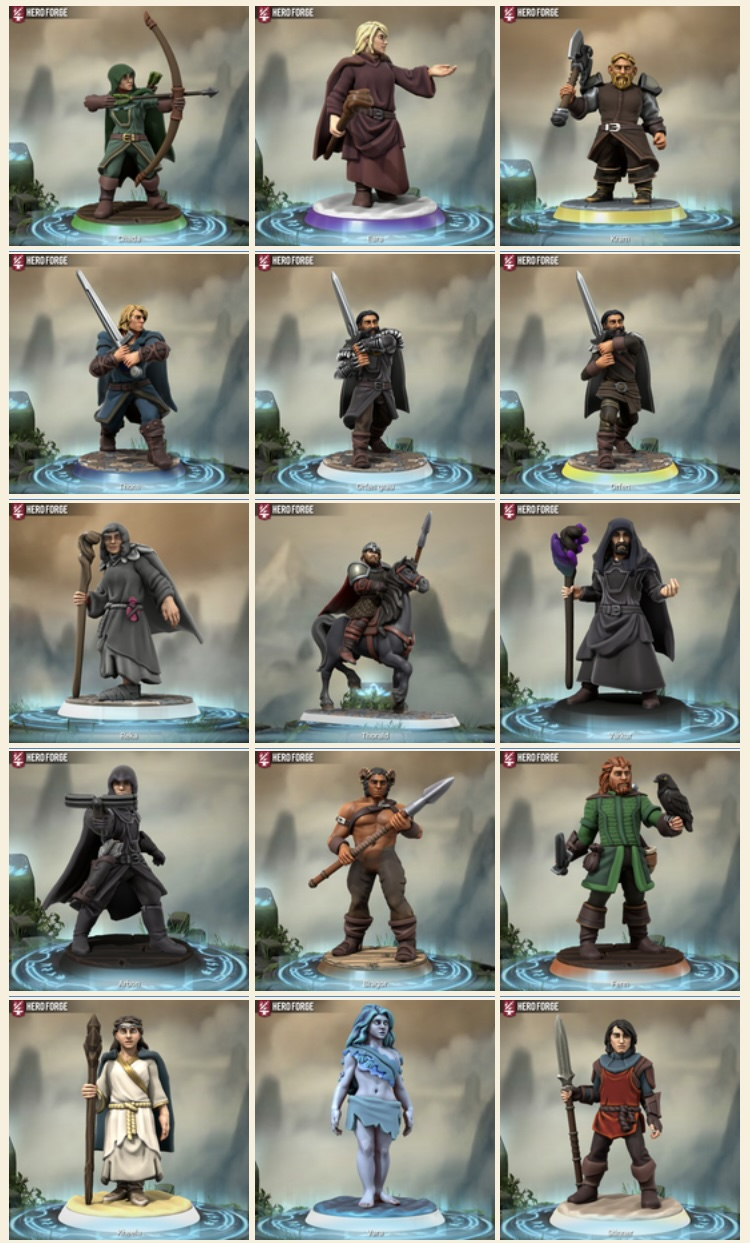
\includegraphics[width=0.3\linewidth]{Das Erbe des Wunderkindes/Bilder/3D mit der Heldenschmiede 1.jpg}
    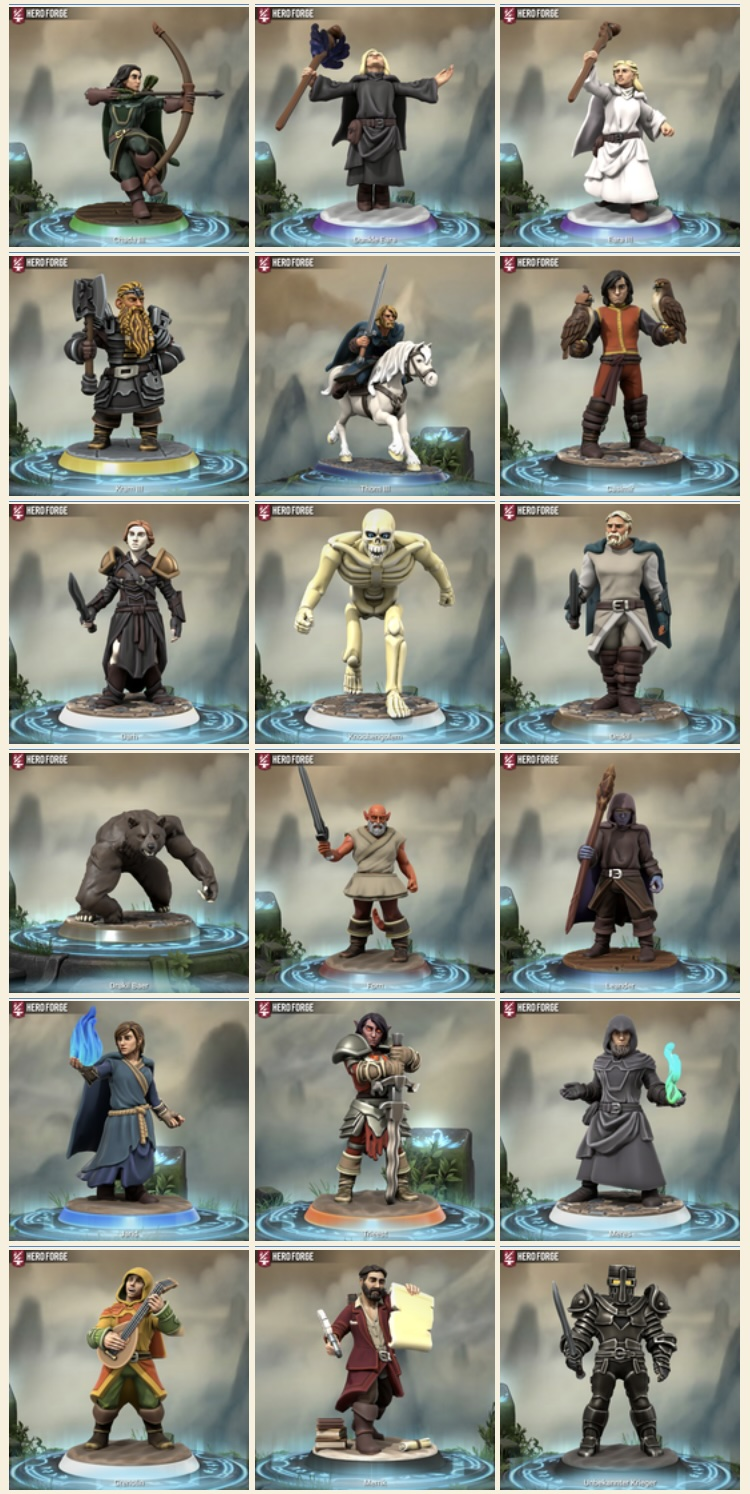
\includegraphics[width=0.3\linewidth]{Das Erbe des Wunderkindes/Bilder/3D mit der Heldenschmiede 2.jpg}\\
    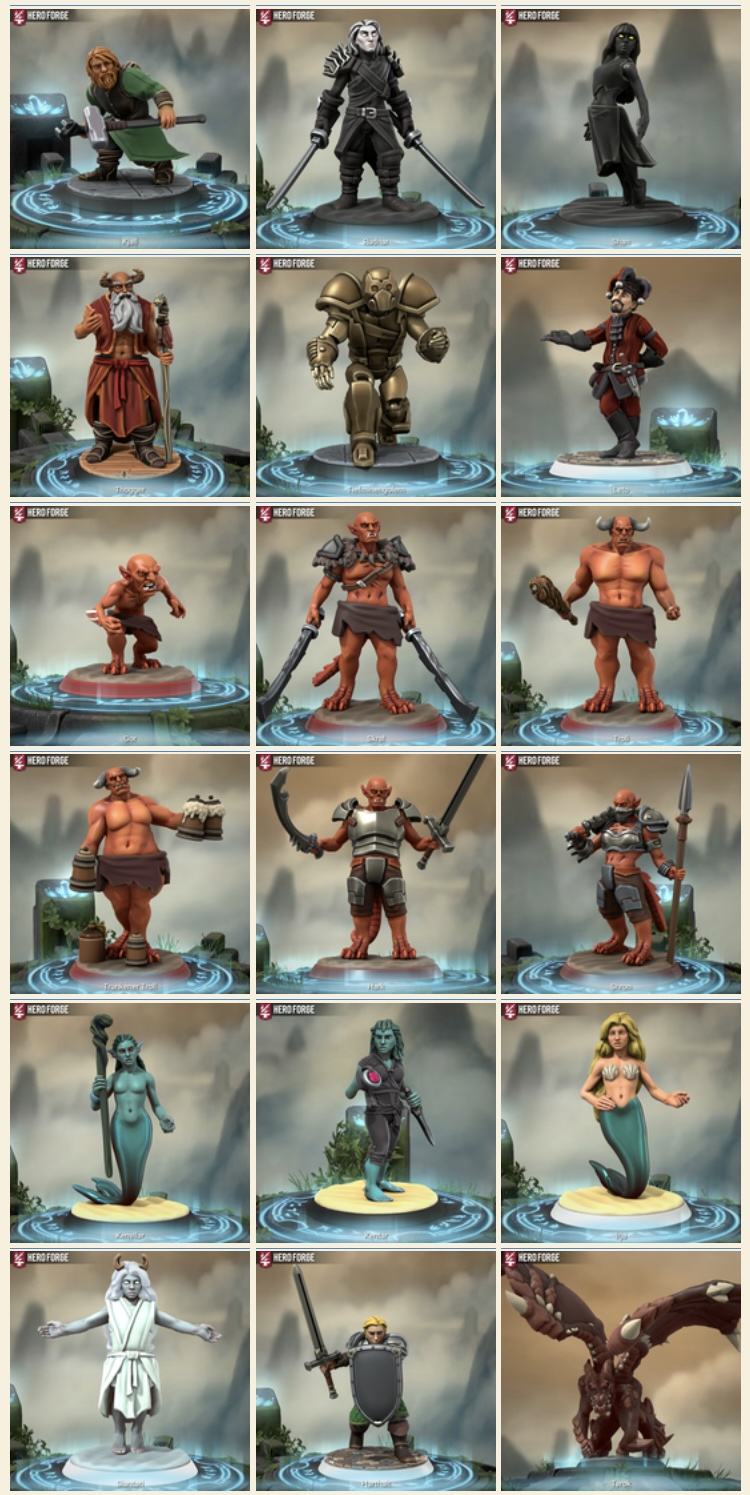
\includegraphics[width=0.3\linewidth]{Das Erbe des Wunderkindes/Bilder/3D mit der Heldenschmiede 3.jpg}
    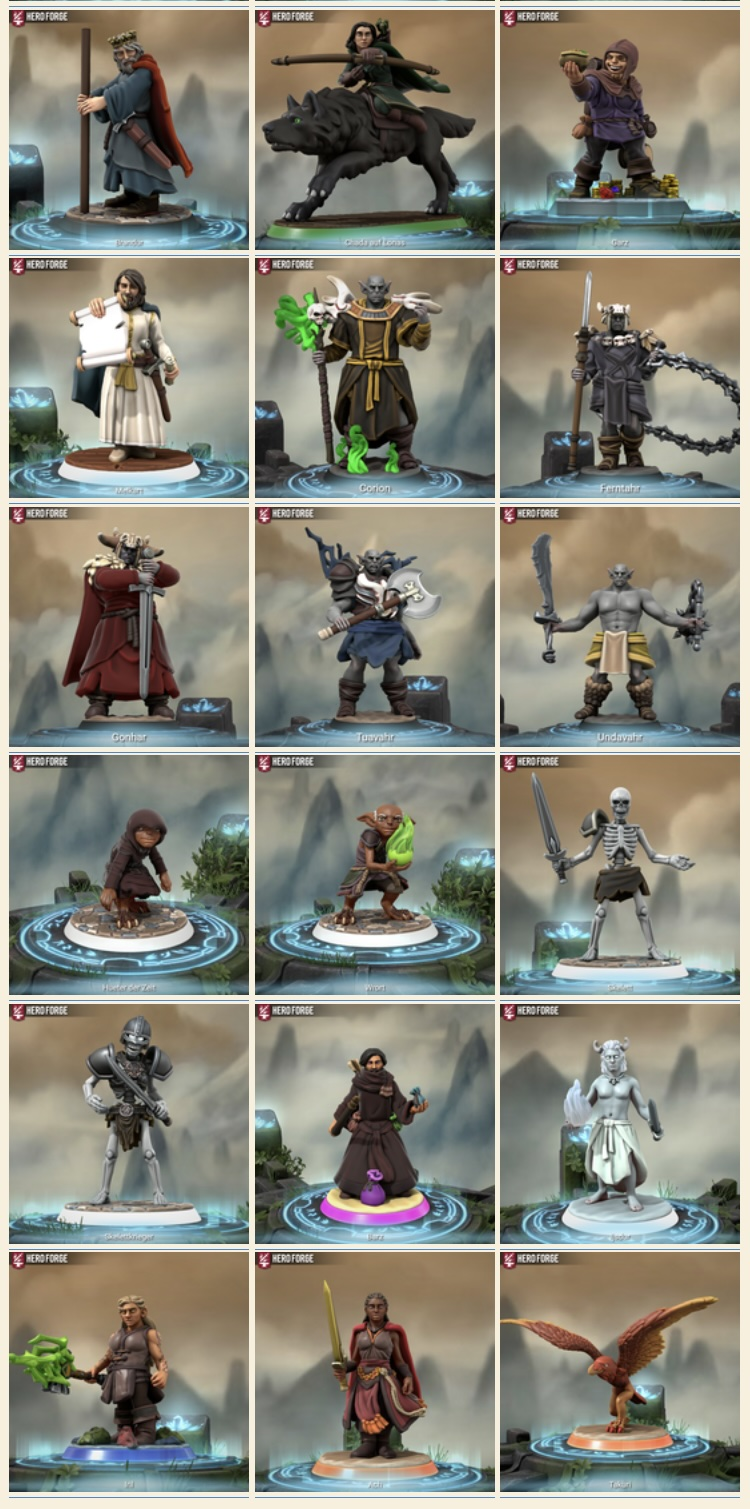
\includegraphics[width=0.3\linewidth]{Das Erbe des Wunderkindes/Bilder/3D mit der Heldenschmiede 4.jpg}
\end{figure}

Hallo liebe Andori,\bigskip

immer mal wieder kam das Thema "3D-Miniaturen für Andor" auf. Solche Figuren hätten sicherlich ihren Reiz, wobei ich die schönen gemalten Charaktere eigentlich doch lieber habe zum Spielen. Nichtsdestotrotz habe ich mal die Heldenschmiede (\url{https://www.heroforge.com/}) angeworfen und ein paar Beispielcharaktere erstellt. Vieles hat natürlich nicht perfekt funktioniert. Ich hab versucht, das beste rauszuholen :D

Drucken lassen werde ich mir keine, es hat mir einfach Spaß gemacht, sie zu designen und ich dachte, ich teile die Bilder mit euch :D

Ich finde die Seite auch ganz praktisch, um für etwaige Bilder auf Fan-Legenden Bild-Modelle von verschiedenen Charakteren zu erstellen, die man dann evtl. mit einem Bildbearbeitungsprogramm noch verfeinern kann.\bigskip

LG

Giftknödel


}